% !TEX root = SystemTemplate.tex

\chapter{System  and Unit Testing}

This section describes the approach taken with regard to system and unit testing. 

\section{Overview}
For both the Android and iOS products, testing needs to be done frequently to ensure quality and desired functionality. We achieve this through writing unit tests for individual units of code, based on predetermined goals.\\


We use a common mnemonic for unit testing, ``A.A.A.'', which stands for Arrange, Act, and Assert. By following this simple pattern, we arrange a test for our predetermined goal (instantiate objects, fill objects with the proper data, etc), then perform our test in the ``act'' portion. Afterwards, we move to the assertion portion, where we validate our finding against our predetermined goal results. From there, we improve our implementation through refactoring and running the test again, repeating the process until we achieve our goal results.\\

After unit testing is complete, we then further validate our findings through a rigorous system test. For this, we emulate a hardware device via a virtual machine connected to the IDE. This allows us to make any configuration changes and UI changes that may be necessary to improve the user experience, and follow a similar refactoring process as our unit testing.\\

Finally, we move on to a true hardware test. The Android and iOS products are deployed to our developers' personal devices and essentially run to break, where we search for any vulnerabilities in design, functionality, and security.

\section{Dependencies}
In both Android and iOS, our testing relies on some sort of framework to help automate and run our unit tests. This includes the ability to generate, run, and refactor unit tests. 

\subsection{Android Testing}
Android Studio has some testing features built-in to the IDE. For individual unit testing, we are utilizing the JUnit framework. This allows us to create class-specific and method-specific tests. Additionally, JUnit works with several mocking frameworks, should we choose to rely on a framework to do so.\\

For system testing in Android, we are able to use the built-in emulator to run a virtual mobile device. Through this, we can see a very close representation to what our app looks like, as well as get a better idea for the desired user experience. After the app is tested on the emulator, we then test it on our personal Android devices to verify our findings from the emulator.

\subsection{iOS Testing}

\section{Test Setup and Execution}
Describe how test cases were developed, setup, and executed.  This section can 
be extremely involved if a complete list of test cases was warranted for the system. 


\begin{table}[tbh]
\caption{The texting Matrix For CrowdControl. \label{testingmatrix}}
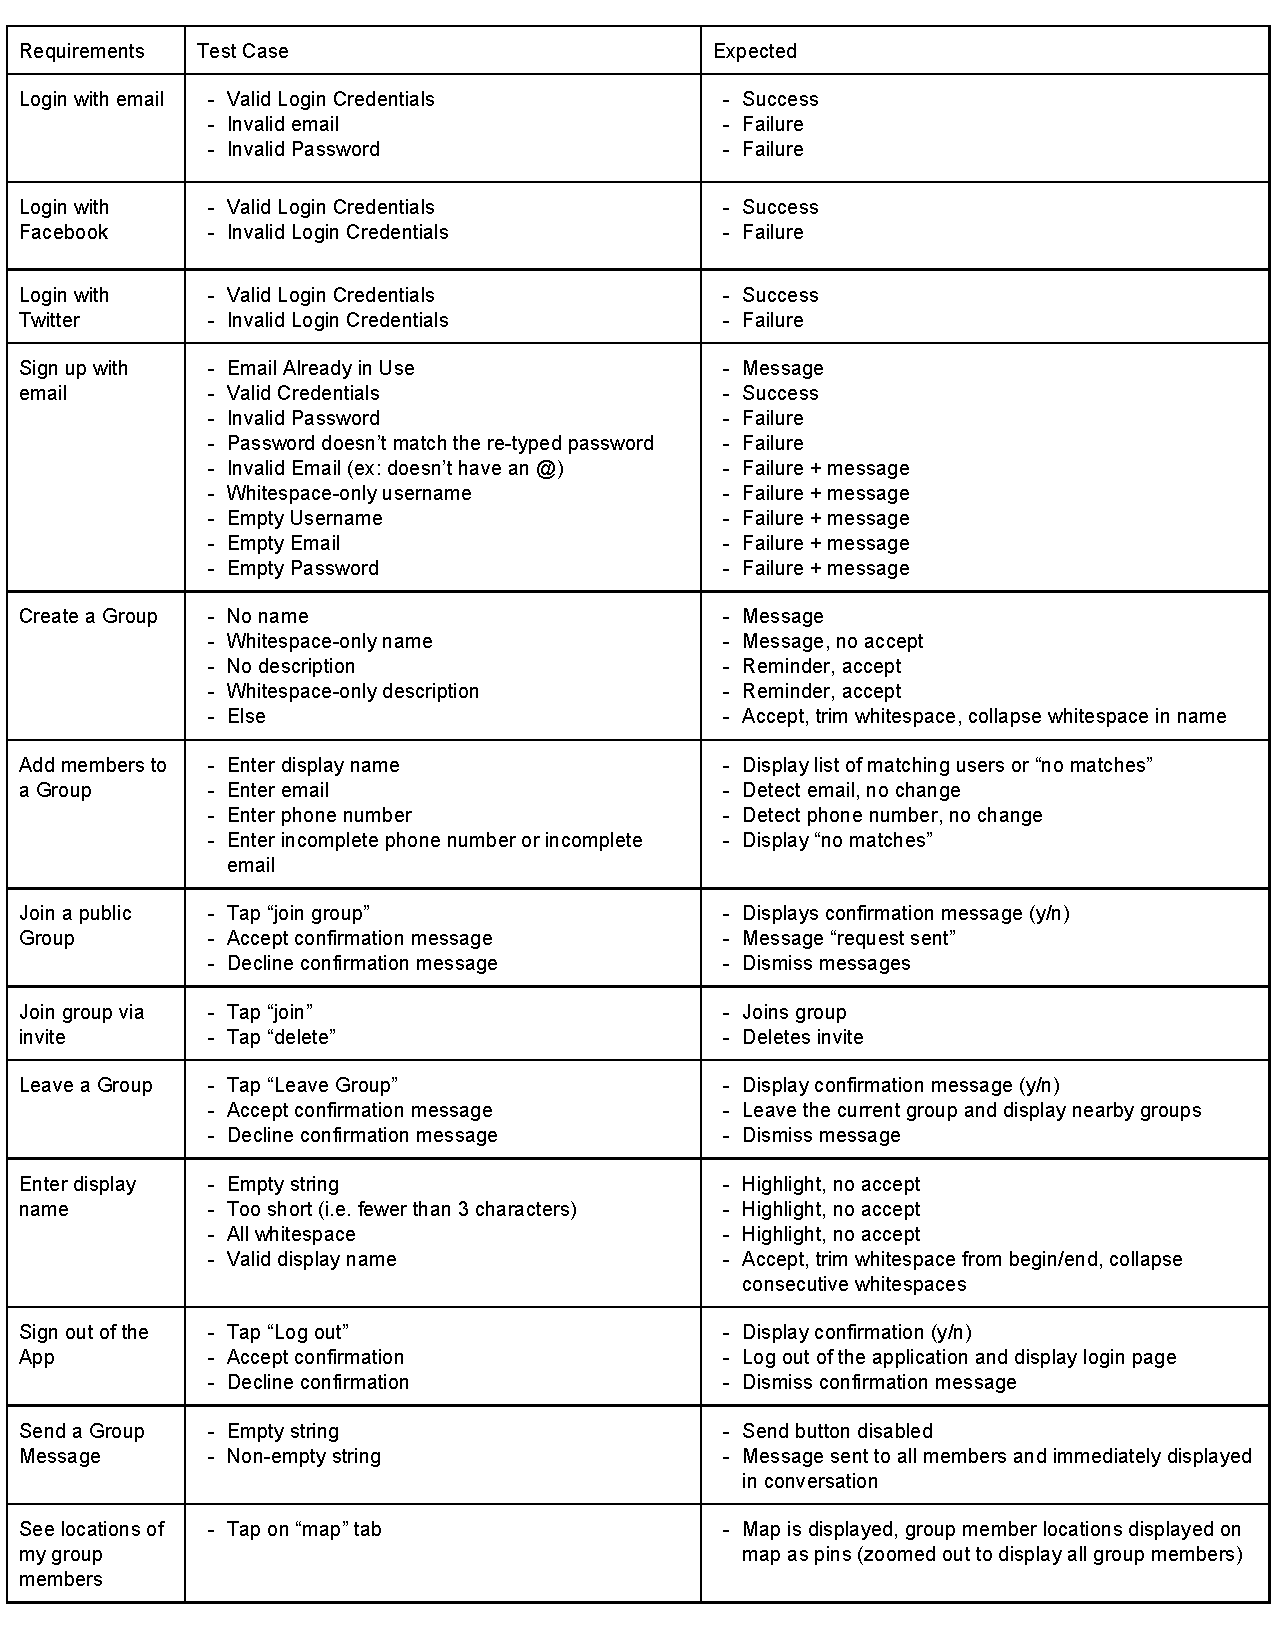
\includepdf{DesignPictures/TestingMatrix.pdf}
\end{table}

